\title{Методы профилирования сборщиков мусора}
%
\titlerunning{Профилирование сборщиков мусора}
\author{Бакрадзе Лиана Георгиевна}
%
\authorrunning{Л.Бакрадзе} % abbreviated author list (for running head)
%
%%%% list of authors for the TOC (use if author list has to be modified)
\tocauthor{Л.Г.Бакрадзе}
%
\institute{Санк-Петербургский государственный университет\\
\email{medeja.bloody@gmail.com}}

\maketitle              % typeset the title of the contribution

\begin{abstract}
В работе рассмотрены некоторые общеупотребимые методы, применяемые для
оценки производительности сборщиков мусора.
\keywords{виртуальные машины, управление памятью, сборка мусора, профилирование}
\end{abstract}
%


\section*{Введение}
В современных системах широко используется динамическое выделение памяти, позволяющее 
выделять память под объекты, размер которых и время жизни неизвестны во время компиляции, 
и освобождать её из-под них. Освобождать и выделять память можно вручную. Но такой
подход влечёт за собой большое количество проблем: утечки памяти, случайное удаление 
используемых блоков памяти, ``висячие'' ссылки, фрагментацию. Для автоматизации управления этим видом 
памяти существуют сборщики мусора. В этом случае выделяется память вручную, а освобождается 
она автоматически. Впервые сборку мусора применили в 1959 году в среде программирования 
на функциональном языке Lisp. Сегодня технология сборки мусора используется, например,
в Java, C\#, OCaml, Haskell.

Подходов к сборке мусора существует довольно много. Для точной сборки мусора необходима 
поддержка среды, так как требуется некоторая модель работы с памятью:
\begin{enumerate}
\item все указатели абстрактные;
\item внутри любой структуры данных возможно определить все указатели.
\end{enumerate}

Когда эти условия нарушаются, применяются консервативные сборщики мусора. Самым известным
сборщиком мусора этого класса является так называемый ``бёмовский''
сборщик мусора\footnote{http://www.hpl.hp.com/personal/Hans\_Boehm/gc/}. 

Для большинства алгоритмов и подходов есть реализации под различные платформы (.Net,
Mono, JVM). Более того, постоянно появлются новые платформы и алгоритмы, а старые 
изменяются и совершенствуются. Поэтому необходимы критерии
и инструменты, позволяющие оценивать эффективность разных реализаций.

Современные платформы поддерживают разные
сборщики мусора. Каждый из этих сборщиков мусора можно настраивать, меняя его параметры,
например, увеличить объём памяти, доступный приложению. 
Необходимы критерии и инструменты оценки и для того, чтобы оценивать
эффективность выбранных параметров для конкретного приложения. 

Определённые алгоритмы обладают определёнными свойствами. С фрагментацией, например, лучше всего 
справляется копирующий сборщик мусора, а для ситуации, когда в программе большая
часть объектов имеет короткое время жизни, больше подойдёт сборка мусора с поколениями (generational).
Сборщик мусора может стать ``бутылочным горлышком'' в работе программы: он может вызываться
неоправданно часто, недостаточно быстро удалять объекты, очень сильно фрагментировать 
память или слишком сильно загружать CPU. Таким образом, просто посчитать общее время 
работы программы с различными реализациями сборщиков мусора недостаточно, нужно 
учитывать и другие факторы. Как важнейшие характеристики работы сборщика мусора выделяют:
объём вычислительных ресурсов, затрачиваемых сборщиком мусора, продолжительность
пауз в работе программы и объём используемой памяти.

Целью данной работы является изучение существующих критериев оценки эффективности сборщиков 
мусора, изучение способов измерения величин, характеризующих работу сборщиков мусора,
а также создание прототипа системы, позволяющей эти величины измерять. 

В качестве целевой платформы выбрана JVM, так как она является одной из самых активно 
развивающихся и распространённых. Существует большое количество языков, у которых 
есть реализации для этой платформы (JPython, Scala\footnote{http://www.scala-lang.org/},
Java, Kotlin\footnote{http://kotlin.jetbrains.org/}).

\section{Существующие критерии оценки эффективности сборщиков мусора}

Традиционный подход к оценке производительности сборщиков мусора состоит в том, чтобы,
запустив определённый набор программ с разными сборщиками мусора, выбрать тот 
алгоритм сборки мусора, при котором время работы наилучшее. Однако, во-первых, набор
тестовых программ может быть далёк от реального пользовательского приложения, во-вторых,
скорость выполнения может быть не самым важным требованием к программе. Например, в системах
реального времени самое важное требование заключается в том, что приложение должно
обязательно давать ответ в течение некоторого промежутка времени. По описанным причинам
при сравнении эффективности различных алгоритмов сборки мусора выделяются и другие критерии,
по которым эти алгоритмы и сравниваются. 

В статье \cite{book:goetz} рассматриваются основные алгоритмы сборки мусора, а также 
приводятся следующие критерии, которыми можно руководствоваться при оценке производительности
сборщиков мусора:
\begin{enumerate}
\item продолжительность пауз в работе приложения, вызванных сборкой мусора;
\item возможность запланировать паузы таким образом,
чтобы улучшить производительность пользовательского приложения;
\item ``отпечаток'' памяти (memory footprint), например, в виде отношения максимальной части динамической 
памяти, занимаемой пользовательской программой, к реальному размеру динамической памяти;
\item количество выгружаемых в виртуальную память страниц;
\item удаление сборщиком мусора данных, используемых пользовательской
программой, из кэш-памяти;
\item потребление ресурсов процессора, например, процент времени центрального процессора,
который тратится на сборку мусора;
\item улучшение расположения пользовательских объектов в памяти с целью уменьшения 
фрагментации;
\item влияние требований сборщика мусора к среде на производительность. 
\end{enumerate}

В \cite{book:Zorn} с помощью разработанной автором системы MARS сравниваются различные 
алгоритмы сборки мусора. Измерения с помощью системы производились в коммерческой системе на языке
программирования Lisp\footnote{https://en.wikipedia.org/wiki/Lisp\_(programming\_language)}.
Система была протестирована на восьми больших приложениях. Для сравнения алгоритмов сборки мусора 
автором были выделены следующие метрики:
\begin{enumerate}
\item производительность сборщика мусора --- параметр, представляющий собой функцию от
времени работы;
\item взаимодействие алгоритма сборки мусора с памятью как на уровне основной памяти, так и кэш-памяти;
\item частота и продолжительность пауз, вызванных работой сборщика мусора.
\end{enumerate}

Разработанная система независимого анализа приложения и сборщика мусора,
описанная в \cite{book:HBench}, предоставляет метрику, которая отражает производительность
пользовательского приложения в условиях работы конкретного сборщика мусора. Эта система
основывается на трёх группах характеристик: характеристики приложения, характеристики 
выделения памяти и характеристики освобождения памяти. К характеристикам приложения
относятся: частота выделения памяти в приложении, частота освобождения памяти в приложении,
возраст объектов, число ссылок на объекты. Характеристика выделения памяти выражается
как функция от состоянии кучи и объёма запрашиваемой памяти, а характеристика освобождения
памяти как функция от трёх величин: фиксированных затрат сборщика мусора (например,
время на инициализацию необходимых ему структур данных), времени, которое тратится
на то, чтобы произвести все необходимые операции с живыми объектами, и, собственно,
времени освобождения памяти.

В аннотации нового сборщика мусора G1\footnote{http://www.slideshare.net/iwanowww/g1-gc-hotspot-jvm}
выделяется три важнейшие характеристики сборщика мусора, отражающие его эффективность:
производительность (как быстро работает программа со сборщиком мусора, как много
вычислительных ресурсов ей требуется), предсказуемость (гарантируется ли, что продолжительность 
пауз, возникающих в приложении при работе мусора, не превысит некоторого известного
интервала времени) и ``отпечаток памяти'' (соотношение динамической памяти, реально
использованной приложением, и общего размера кучи, а также соотношение памяти в различных 
областях кучи).


\section {Сборка мусора в Hotspot JVM}

Различные приложения предъявляют разные требования к работе сборщика мусора: для некоторых важно минимизировать
продолжительность пауз в работе сборщика мусора. Для некоторых важна максимальная 
производительность и скорость исполнения, а некоторые должны использовать минимально
возможное количество памяти. К тому же виртуальная машина JVM может быть запущена
как на мощных серверах с большим объёмом памяти и с несколькими процессорами, так и на 
обычных клиентских машинах. Поэтому виртуальная машина для настольных компьютеров и серверов
Hotspot JVM поддерживает несколько различных алгоритмов сборки
мусора.

Все сборщики, которые есть в Hotspot JVM на настоящий момент, относятся к типу сборщиков мусора
с поколениями. Их работа основывается на так называемой ``слабой гипотезе о поколениях'':
большинство объектов живут недолго и количество ссылок на них мало. Память делится на области, называемые
поколениями (generations). В Hotspot JVM два основных поколения: младшее поколение (young generation)
и старшее поколение (old generation).
В младшем поколении размещаются новые объекты. По размеру оно меньше, чем 
старшее, как следствие, оно быстро заполняется, и сборки мусора в этой
области проводятся чаще. Так как большинство объектов в области младшего поколения
являются мусором, то сборки мусора
(они называются малыми сборками) происходят быстро и очень эффективно. В область старшего поколения
перемещаются объекты,
пережившие несколько сборок мусора. Эта область заполняется медленнее и имеет больший объём,
поэтому сборки мусора (большие сборки мусора) в ней происходят редко, но зато они занимают
много времени из-за того,
что все объекты, как правило, имеют большой объём. Учитывая особенности сборки мусора 
в каждой из областей, для каждой области подбирается оптимальный алгоритм.

На машинах клиентского типа (они имеют небольшой объём вычислительных ресурсов) по
умолчанию используется последовательный сборщик мусора --- SerialGC, его также 
называют однопоточным сборщиком мусора. Во время работы последовательного сборщика
мусора все потоки приложения приостанавливаются, то есть в процессе работы приложения
возникает так называемая ``stop-the-world'' пауза. Сборка мусора выполняется только 
одним потоком (это свойство и дало сборщику мусора название ``последовательный'').
Для младшего поколения используется копирующий сборщик мусора. Суть его работы заключается
в том, что вся доступная память в этой области делится на три части.
В первой части создаются все новые объекты. Когда она заполняется,
запускается малая сборка мусора.
При этом во второй части уже содержатся объекты, пережившие
одну сборку мусора. Сборщик мусора обходит все живые новые объекты (они размещены в первой части) и не пережившие заданного числа сборок мусора 
живые объекты во второй части. Он перемещает их в третью часть.
Оставшиеся живые объекты перемещаются в область старшего поколения. В конце малой сборки мусора
части вторая и третья части меняются местами, первая часть пуста, новая 
новая третья часть тоже пуста. В старшем поколении сборка мусора происходит с использованием 
маркирующе-сжимающего
(Mark-and-Compact) алгоритма, который имеет три фазы. В фазе пометки (Mark) помечаются
все живые объекты, в фазе освобождения (Sweep) все непомеченные объекты удаляются, 
а в фазе уплотнения (Compact) все живые объекты перемещаются в начало области старшего, 
в результате чего свободная память после очистки представляет собой непрерывную область. 

В Hotspot JVM можно также включить параллельный сборщик мусора отдельно как для младшего поколения, 
так и для старшего. При этом будут использоваться те же алгоритмы, которые
использует SerialGC, однако в соответствующем поколении сборка мусора будут разделяться между несколькими 
потоками, что сделает паузы, вызываемые сборками мусора, короче.

Многие приложения очень чувствительны к stop-the-world паузам в работе, и для таких приложений
важно эти паузы минимизировать. Сборщик мусора, который частично решает эту проблему — 
Concurrent Mark Sweep GC (CMS), его также называют фоновым сборщиком мусора.
Если выбран CMS, то в младшем поколении по умолчанию используется параллельный копирующий
сборщик мусора, но можно выбрать и однопоточный. Цикл работы CMS состоит из нескольких этапов.
Во время этапа начальной маркировки сборщик мусора находит все так называемые 
корневые ссылки (roots). К ним относятся ссылки, сохранённые в регистрах и на стеках. На время
этого этапа приложение ненадолго приостанавливается. Следующий этап --- этап одновременной
маркировки, во время которого сборщик мусора помечает все ссылки, до которых 
можно добраться по ссылкам из корневых, то есть все живые объекты. Однако
во время этого этапа могли быть созданы новые объекты или изменены старые, так как приложение
не приостанавливается. Поэтому следующим этапом осуществляется повторная маркировка, чтобы
сборщик мусора проверил все объекты, которые были созданы или изменены во время предыдущего
этапа. И, наконец, последним этапом CMS, не приостанавливая приложение, удаляет все
непомеченные объекты. Этот этап называется этапом одновременной очистки.

В Oracle JDK 7 появился ещё один сборщик мусора --- Garbage-First (G1). Этот сборщик 
мусора предназначен в первую очередь для многопроцессорных систем с большим объёмом памяти,
он является как фоновым, так и паралелльным и обладает высокой предсказуемостью работы.
G1 также является сборщиком мусора с поколениями, но вся память делится на области 
одинакового размера, называемые регионами. Младшее поколение размещается в некотором
наборе регионов (они не обязательно должны быть смежными), которые делятся на области размещения новых
объектов и области размещения объектов, переживших несколько сборок мусора. 
Старшее поколение также представлено набором регионов. Те объекты,
размер которых превосходит размер одного региона, хранятся в нескольких смежных регионах.
При достижении некоторой пороговой занятости динамической памяти запускается процесс
фоновой маркировки, во время которого G1 обновляет информацию о количестве живых объектов
по регионам и освобождает память в регионах, в которых не осталось живых объектов. Во
время stop-the-world пауз сборщик мусора проверяет корректность фоновой маркировки.
На ряду с понятием малых сборок мусора появилось понятие
смешанных сборок мусора. Смешанная сборка мусора проводится в определённом
наборе регионов, который включает младшее поколение и часть регионов старшего поколения, при 
этом выбираются те регионы из старшего поколения, в которых больше всего непомеченных объектов.
Сборка мусора происходит копированием живых объектов в область переживших несколько сборок мусора объектов,
включающую свободные регионы старшего поколения. Возможность независимо 
собирать регионы обеспечивается хранением информации о местонахождении ссылок на объекты
из региона (Remembered Set). Такая информация хранится для ссылок между регионами старшего поколения
и из старшего поколения в младшее.

Каждый из описанных сборщиков мусора имеет свои настраиваемые параметры, например, для G1
можно задать желаемые частоту и продолжительность stop-the-world пауз, а для SerialGC
можно увеличить размер младшего поколения. 

\section{Существующие инструменты оценки\\эффективности сборщиков мусора в JVM}
Для оценки эффективности работы сборщика мусора можно использовать инструменты, 
предназначенные для сбора характеристик работы программы, --- профилятор. Рассмотрим 
один из самых популярных профиляторов для JVM --- VisualVM\footnote{http://visualvm.java.net/}.
С его помощью удобно
следить за тем, какой объём ресурсов потребляет сборщик мусора. Можно посмотреть,
какой процент CPU потребляет пользовательское приложение и сколько из них приходится
на активность сборщика мусора. Можно посмотреть соотношение между использованной
приложением памятью и общим размером памяти. Также, установив плагин VisualGC, можно
посмотреть на распределение памяти в каждой из областей кучи. Однако пользоваться 
профайлером для оценки таких характеристик эффективности сборщика мусора, как, например,
продолжительность пауз, очень неудобно, потому что профайлер не предоставляет для них 
никакого численного измерения. Не все сборщики мусора в полной мере поддерживаются 
VisualVM. Например, если запустить приложение с G1 сборщиком мусора, то посмотреть распределение
памяти в различных областях нельзя.

Ещё одним инструментом, который можно применить для оценки эффективности сборщика мусора,
является GCHisto\footnote{https://java.net/projects/gchisto/}. Он визуализирует журналы
с записями о событиях (логи), генерируемые JVM. Этот инструмент предоставляет различную 
информацию о stop-the-world паузах в работе приложения: количество пауз, их общая продолжительность,
продолжительность самой долгой и самой короткой паузы. Также можно посмотреть общее количество
сборок мусора и количество сборок мусора каждого типа. Для всей предоставляемой информации
имеются различные способы её количественного выражения (например, количество малых сборок мусора
и процент малых сборок мусора от общего количество сборок мусора) и графического представления
(графики, гистограммы). Однако этот инструмент имеет большое количество недостатков:
во-первых, он уже в течение двух лет заброшен, во-вторых, он не проводит никаких
измерений, связанных с памятью (например, объём использованной приложением памяти), в-третьих,
он поддерживает не все сборщики мусора, реализованные в JVM.
% У заключения нет номера главы

\section{Описание системы оценки производительности\\сборщиков мусора}

В процессе работы было рассмотрено три способа профилирования сборщиков мусора:
методы класса Runtime, интерфейс профилирования Java Virtual Machine Tool Interface
(JVMTI)\footnote{http://docs.oracle.com/javase/7/docs/technotes/guides/jvmti/} и анализ
логов виртуальной машины.

С помощью методов класса Runtime\footnote{http://docs.oracle.com/javase/7/docs/api/}
был написан простой класс Monitor, который выводит текущее время, количество свободной памяти,
общее количество памяти, общее количество объектов, количество живых объектов и 
количество мёртвых объектов (мусора). Однако такой способ профилирования, во-первых,
не позволяет измерить многие важнейшие характеристики работы сборщика мусора (продолжительность
пауз, например), во-вторых, требует изменения приложения (перегрузки конструкторов и 
метода finalize).

Интерфейс профилирования JVMTI предоставляет много возможностей для профилирования
работы сборщика мусора. Профилирование осуществляется с помощью специальной программы,
которая называется VM-агентом, эта программа может обрабатывать генерируемые JVM
события, например, запуск и окончание работы сборщика мусора или операции выделения
памяти. VM-агент запускается в том же процессе и адресном пространстве, что и сама
JVM, поэтому плохо написанный агент может привести к тому, что JVM завершит свою
работу с ошибкой. Был написан небольшой VM-агент, позволявший получать информацию
о продолжительности stop-the-world пауз в работе приложения и количестве вызовов сборщика
мусора. Однако не все сборки мусора генерируют соответствующие события, поэтому таким способом не получить
информацию о работе всех доступных в JVM сборщиков мусора.

И, наконец, третий часто применяющийся способ --- анализ логов JVM. Именно он впоследствии
и был выбран для создания прототипа системы оценки.

Система написана на языке Python\footnote{http://www.python.org/} и представляет собой
библиотеку, функциями которой можно пользоваться после её подключения. Для получения
статистики необходимо запустить приложение с несколькими специальными ключами: 
\begin{enumerate}
\item выбор сборщика мусора\footnote{http://www.oracle.com/technetwork/java/javase/tech/vmoptions-jsp-140102.html};
\item \textit{-XX:+PrintGCDetails} --- вывод логов сборщика мусора;
\item \textit{-Xloggc:имя файла} --- перенаправление логов сборщика мусора в файл.
\end{enumerate}
После этого в зависимости от выбранного сборщика мусора требуется вызвать одну из
четырёх функций: \textit{parseSerialGC}, \textit{parseParGC}, \textit{parseCMS}
и \textit{parseG1}. Каждой из этих функций в качестве параметров передаётся имя файла 
с логами и список --- структура данных, в которой будет сохранена информация о
вызовах сборщика мусора, этот список передаётся на вход другим функциям системы.

С помощью системы можно получать следующую информацию о работе сборщика мусора:
\begin{enumerate}
\item процент времени работы сборщика мусора от общего времени работы приложения;
\item общее время работы сборщика мусора в секундах;
\item количество вызовов сборщика мусора;
\item максимальная продолжительность stop-the-world паузы в работе приложения;
\item средняя продолжительность stop-the-world паузы в работе приложения;
\item максимальный процент использованной памяти от общего объёма памяти;
\item минимальный процент использованной памяти от общего объёма памяти;
\item средний процент использованной памяти от общего объёма памяти;
\item количество малых и больших сборок мусора для SerialGC, ParallelGC и G1;
\item количество фаз, во время которых осуществлялась сборка мусора, и фаз, во время
которых сборка мусора не осуществлялась, для СMS.
\end{enumerate}


Также система предоставляет возможность получить графическое представление
продолжительности работы сборщика мусора и соотношения использованной и общей 
памяти. Для построения графиков
используется программа gnuplot\footnote{http://www.gnuplot.info/}.
Для того, чтобы получить один из графиков для определённого сборщика 
мусора, необходимо вызвать соответствующую функцию, передав ей в качестве параметров
имя будущего графика и список с информацией о сборках мусора. Функция
сгенерирует скрипт data.sh на bash\footnote{https://en.wikipedia.org/wiki/Bash\_(Unix\_shell)}, который можно изменить, если необходимо.
Скрипт нужно пометить как исполняемый файл(например,
с помощью программы \textit{chmod}) и запустить, на выходе получится готовый график.

\section{Результаты}
Разработанная система оценки была протестирована на готовом тесте, представленном 
на сайте ``бёмовского'' сборщика мусора\footnote{http://www.hpl.hp.com/personal/Hans\_Boehm/gc/gc\_bench/GCBench.java}.
Тестовая программа создаёт двоичные деревья\footnote{http://en.wikipedia.org/wiki/Binary\_tree}
различной глубины. Выделенная под эти деревья память впоследствии должна быть освобождена сборщиком мусора.


В таблице~\ref{table:serialgc} приведены результаты измерений для тестовой программы, запущенной со сборщиком мусора по умолчанию (SerialGC).
В таблице~\ref{table:g1} приведены результаты измерений для тестовой программы, 
запущенной со сборщиком мусора G1. Для этой программы сборщик мусора G1 оказался
более эффективным, так как и продолжительность stop-the-world пауз, и частота вызовов 
сборщика мусора для него меньше, а соотношения использованной памяти к общей памяти
примерно одинаковы.

\begin{table}[h!]
\caption {Результаты измерений для SerialGC}
\label{table:serialgc}
\begin{center}
\begin{tabular}{|l|l|}
\hline
\multicolumn {1}{|c|}{Величина} & \multicolumn {1}{|c|}{Значение величины}\\
\hline
средняя продолжительность паузы & 0.014 сек\\
\hline
максимальная продолжительность паузы & 0.170 сек\\
\hline
количество вызовов сборщика мусора & 22\\
\hline
количество больших сборок мусора & 2 \\
\hline
количество малых сборок мусора & 20 \\
\hline
общее время работы сборщика мусора & 0.321 сек\\
\hline
процент времени работы сборщика мусора & 3.620 \%\\
\hline
максимальный процент использованной памяти & 78.214 \%\\
\hline
минимальный процент использованной памяти & 10.401 \%\\
\hline
средний процент использованной памяти & 32.069 \%\\
\hline
\end{tabular}
\end{center}
\end{table}

\begin{table}[h!]
\caption {\label{table:g1}Результаты измерений для G1}
\begin{center}
\begin{tabular}{|l|l|}
\hline
\multicolumn{1}{|c|}{Величина} & Значение величины\\
\hline
средняя продолжительность паузы & 0.015 сек\\
\hline
максимальная продолжительность паузы & 0.026 сек\\
\hline
количество вызовов сборщика мусора & 7\\
\hline
количество больших сборок мусора & 0 \\
\hline
количество малых сборок мусора & 7 \\
\hline
общее время работы сборщика мусора & 0.109 сек\\
\hline
процент времени работы сборщика мусора & 1.415 \%\\
\hline
максимальный процент использованной памяти & 85.840 \%\\
\hline
минимальный процент использованной памяти & 10.619 \%\\
\hline
средний процент использованной памяти & 36.914 \%\\
\hline
\end{tabular}
\end{center}
\end{table}

На рис.\ref{pic:serialmem} представлено соотношение использованной и общей памяти
при работе SerialGC, а на на рис.\ref{pic:g1mem} при работе G1. Зелёным цветом показано
количество использованной памяти в программе в килобайтах в зависимости от времени (в секундах),
а красным цветом количество общей памяти. Участки резкого убывания на кривой, показанной красным цветом,
соответствуют вызовам сборщика мусора.

\begin{figure}
%\centering
\caption{\label{pic:serialmem}Соотношение использованной и общей памяти при работе SerialGC}
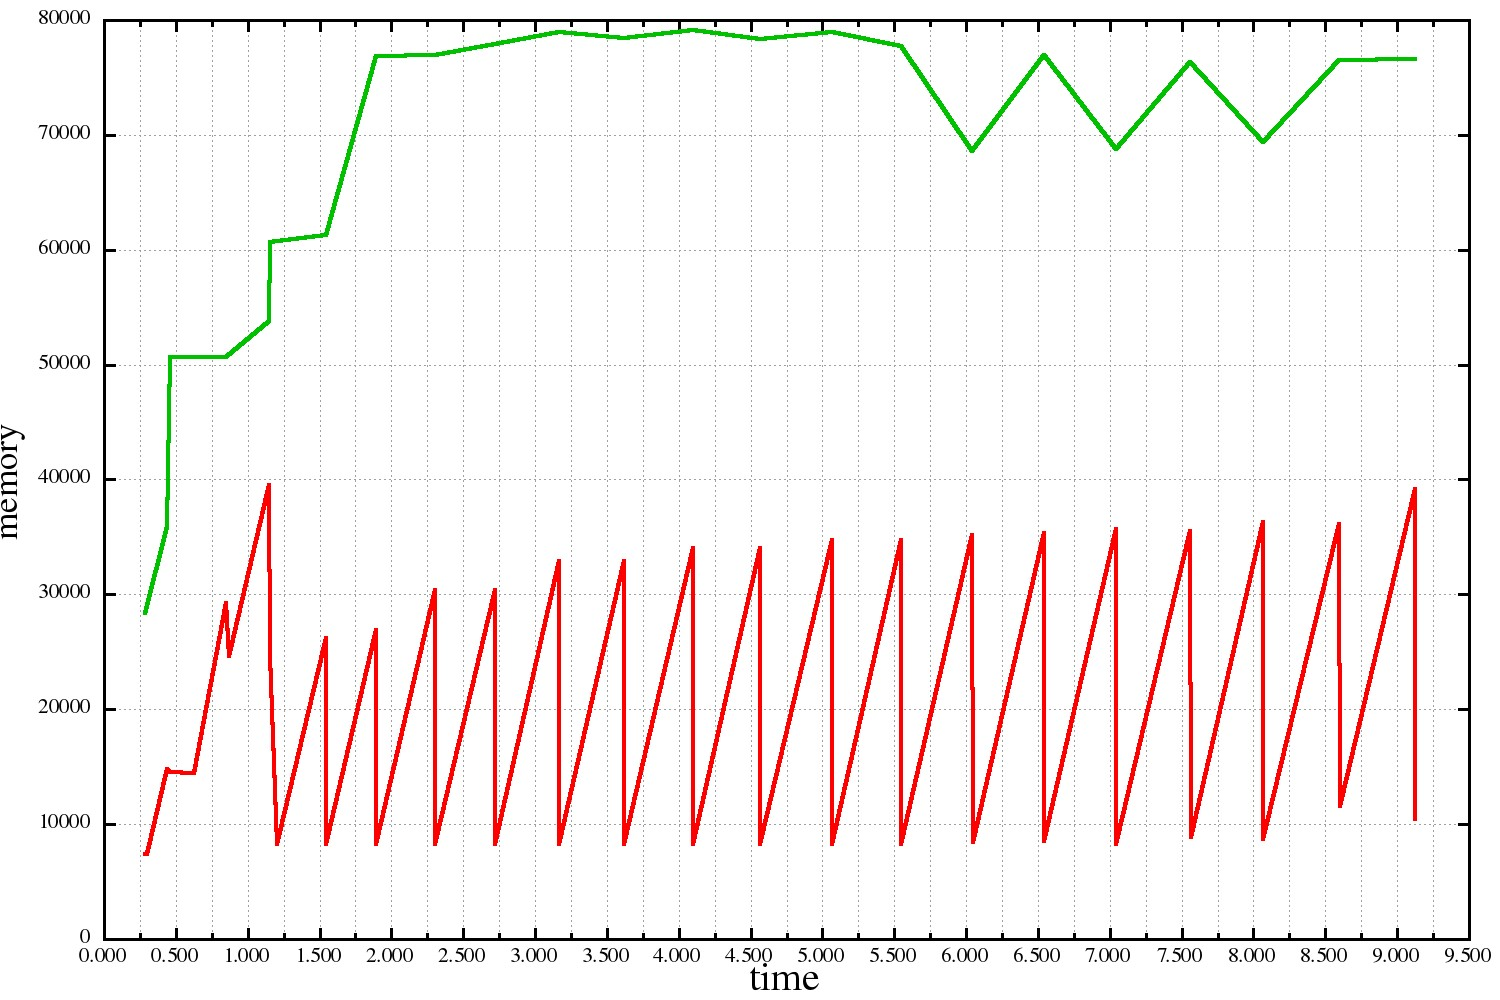
\includegraphics[width=1\linewidth]{Bakradze/serialmem.jpg}
\end{figure}


\begin{figure}
\centering
\caption{\label{pic:g1mem}Соотношение использованной и общей памяти при работе G1GC}
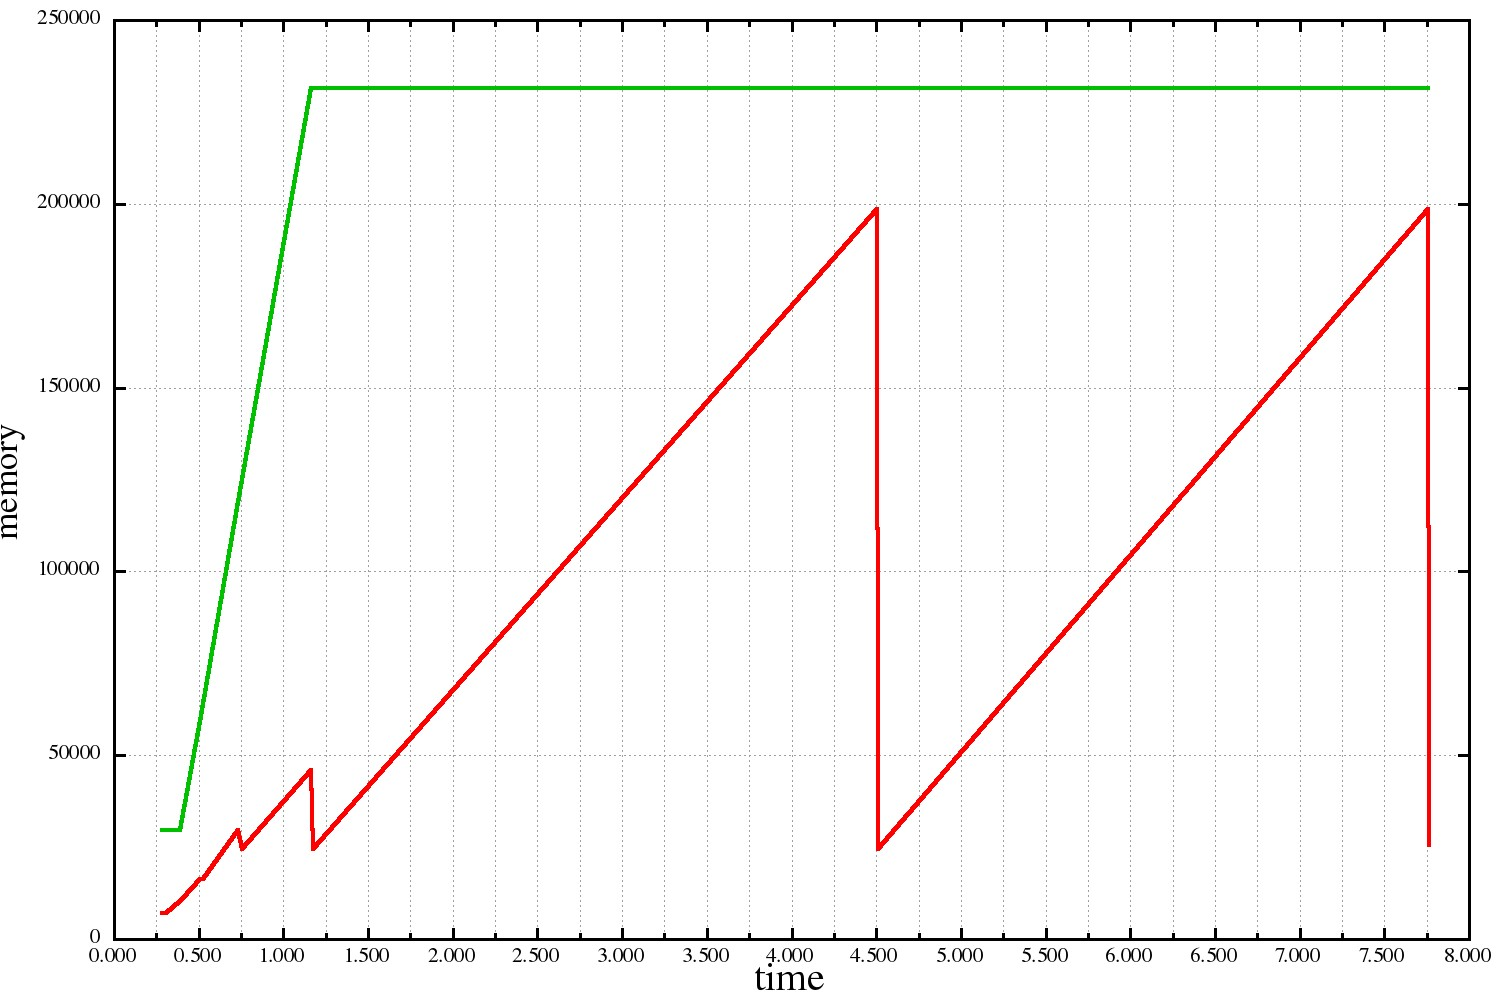
\includegraphics[width=1\linewidth]{Bakradze/g1mem.jpg}
\end{figure}

\section*{Заключение}
\addcontentsline{toc}{section}{Заключение}

В данной работе представлены различные критерии оценки производительности сборщиков мусора,
а также обзор поддерживаемых Hotspot JVM сборщиков мусора и существующих инструментов,
которые можно использовать для оценки их эффективности.

Изучены основные способы профилирования JAVA-приложений: методы класса Runtime, интерфейс
профилирования JVM JVMTI и анализ логов JVM. Были опробованы все способы,
из них выбран наиболее подходящий для данной задачи --- анализ логов JVM.

Создан прототип системы, позволяющей проводить измерения. Система поддерживает все доступные на данный
момент в Hotspot JVM сборщики мусора и предоставляет следующую информацию об их работе: характеристики, связанные
со временем работы (например, продолжительность stop-the-world пауз в работе приложения), и
характеристики, связанные с памятью (например, соотношение между реально использованной 
памятью и общим объёмом памяти), а также некоторые другие характеристики (например,
количество вызовов сборщика мусора и частота его вызовов). Для времени работы сборщика 
мусора и распределения памяти в программе есть возможность их визуализации в виде
графика.

\begin{thebibliography}{99}
\bibitem{book:goetz}
Brien Goetz. A Brief History of Garbage Collection //
Java Theory and Practice, 2003.

\bibitem{book:Zorn}
Benjamin G. Zorn.
Comparative Performance Evaluation of Garbage Collection Algorithms.
Computer Science Division Department of Electrical Engineering and Computer Sciences University of California, Berkeley, California, 1989.

\bibitem{book:HBench}
Xiaolan Zhang, Margo Seltzer.
HBench: JGC --- An Application-Specific Benchmark Suite for Evaluating JVM Garbage Collector Performance. 2001.
\end{thebibliography}
